\title{Ohjelmointikielet ja -paradigmat 2017}
\author{
  Sakari Sn\"all 507267 \\
  Antti Vainikka 510575
\\
}
\date{\today}

\documentclass[12pt]{article}

\usepackage[utf8]{inputenc}
\usepackage{listings}
\usepackage{graphicx}
%\usepackage{listings,mdframed,xcolor}
\begin{document}

\lstnewenvironment{code}[1]
{}
{}
% 
%\renewcommand{\lstlistingname}{Ohjelmakoodi}
%\definecolor{codeBackground}{rgb}{0.9, 0.9, 0.8}
%\lstnewenvironment{code}[1][]{%
%  \lstset{
%    moredelim=**[is][\bfseries]{|}{|},%
%    moredelim=**[is][\itshape]{*}{*},% 
%    numbers=left,%
%    caption={#1},%
%    label=#1
%    }%
%\mdframed[backgroundcolor=codeBackground,shadow=true,shadowsize=2pt,shadowcolor=black!30]%
%}
%{%
%  \endmdframed
%  \ignorespaces
%}

\maketitle

\newpage

\section{Johdanto}
Toteutimme harjoitustyön kolmannen tehtävän.
Valitsimme toteutettavaksi peliksi pokerin koska järkevän toteutuksen tekeminen tutustuttaisi meidät kielen tapaan luoda struktuureita,
lukea syötettä standardista syöteputkesta ja joutuisimme toteuttamaan pelijatkumon funktionaalisesti. Alkuperäisen tietämyksemme perusteella pelin ohjelmoiminen on funktionaalisesti vaikeampaa verrattuna imperatiiviseen tapaan ohjelmoida, koska peleissä on yleensä tila, jota pitää muuttaa usein. Useat peliohjelmointiin liittyvät kirjat ja artikkelit käyttävät olio-ohjelmoinnin paradigmaa, Pelien osat ovat yleensä helpompia hahmottaa kun ne jaetaan yksittäisiin olioihin, joilla on jokin tietty funktio. Ohjelmointityö antaa meille tuntumaa miksi funktionaalinen paradigma ei ole suosittu ainakaan pelien ohjelmoinnissa.

\newpage
\section{Funktionaalinen paradigma}
Funktionaalinen paradigma on deklaratiivisten ohjelmointiparadigmojen luokkaan kuuluva ohjelmointiparadigma. Funktionaalisen paradigman omainaisuuksia ovat esimerkiksi muuttumattomat tietorakenteet ja laiska laskenta. Muuttumattomilla tietorakenteilla tarkoitetaan yleensä yksinkertaisuudessaan sitä, että mikäli halutaan esittää jokin asia muuttuneena, sille luodaan uusi tietorakenne (muuttuja tai funktio esimerkiksi). Laiskalla laskennalla puolestaan tarkoitetaan sitä, että mitään ei lasketa ennen kuin on pakko ja mitään ei lasketa kahdesti.

\subsection{Matemaattinen lähtökohta}
Funktionaalisessa ohjelmoinnissa pyritään kuvaamaan ongelma matemaattisesta näkökulmasta käyttäen funktioita ja lausekkeita. Tietorakenteet ovat usein listoja ja niiden yhdistelmiä. Funktiot pyritään pitämään tarkkaan määriteltyinä ja sivuvaikutuksettomina, eli sellaisina etteivät ne ole riippuvaisia globaalista datasta ja tuottavat aina saman lopputuloksen samoilla lähtöarvoilla.

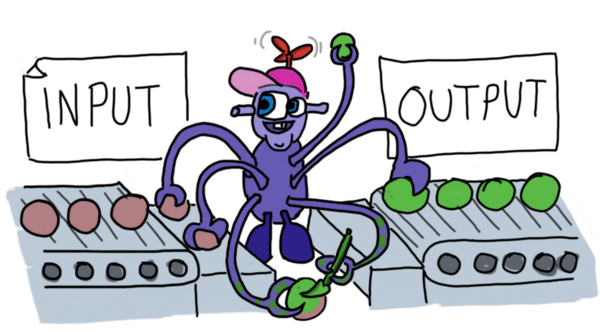
\includegraphics[width=\textwidth]{puhdasfunktio.png}


\subsection{Kontrollivuo}
Funktionaalisen ohjelmoinnin matemaattisuus ilmenee myös siten, että funktioiden suoritusjärjestys ohjataan rekursioiden ja peräkkäisten funktioiden avulla, kun taas imperatiivisessa ohjelmoinnissa ohjaus toimii ehtolauseilla ja iteraatioillai. Funktionaalisilla ohjelmilla ei ole varsinaisesti tilaa kuten proseduraalisissa ohjelmissa, vaan niiden kontrollivuo muodostuu suoraan lausekkeista, funktiokutsuista ja niiden välisistä riippuvuuksista. Koska funktionaalisessa ohjelmoinnissa ei ole monimutkaisia ehtolauseita vaan ohjaus tapahtuu peräkkäisillä funktion kutsuilla on ohjelman toiminta helpommin ennustettavissa.


\subsection{Funktionaaliset ohjelmointikielet}
On vaikea määrittää onko ohjelmoinkieli funktionaalinen vai ei. Useimmissa ohjelmointikielissä on olemassa mahdollisuus luoda anonyymeja funktioita ja sen pohjalta on vedetty johtopäätös, että kieli olisi funktionaalinen. Esimerkiksi Java 8:aa kutsutaan funktionaaliseksi, koska siihen lisättiin lyhenne paikallaan luodulle objektille, joka toteuttaa jonkin rajapinnan.
Funktionaaliset ohjelmointikielet voidaan jakaa kuitenkin puhtaasti funktionaalisiin ja epäpuhtaisiin. Puhtaus funktionaalisissa ohjelmointikielissä viittaa siihen voidaanko kielessä aiheuttaa sivuvaikutuksia. 
Täysin funktionaalisia ohjelmointikieliä on esimerkiksi Haskell ja Clear. ML pohjaiset kielet ovat funktionaalisia mutta esimerkiksi standardissa ML:ssä ja Ocamlissa voidaan asettaa muuttujalle arvo.
Jos halutaan olla tarkkoja niin myös Haskelissa tapahtuu sivuvaikutuksia koska esimerkiksi tekstin tulostaminen sisältää sivuvaikutuksen. Täydellisesti sivuvaikutuksellisessa ohjelmassa ei kuitenkaan ole järkeä koska tarpeeksi tehokas kääntäjä voisi tuottaa ohjelman, joka ei suorita mitään koska sivuvaikutuksia ei tehdä.



%esimerkki funktionaalisesta loopista schemellä
\begin{lstlisting}
(let loop ((n 0))
   (cond
      ((= n 10))
      (#t
       ...
       (loop (+ n 1)))))      
\end{lstlisting}
%esimerkki imperatiivisesta loopista
\begin{lstlisting}
for(int n = 0; n < 10; n++) {
        ...
}
\end{lstlisting}


\subsection{Sulkeumat objektien sijaan}
Ohjelmointikielissä joissa funktioon voidaan sisällyttää ympäristö (closure), pystytään triviaalisti toteuttamaan objektisysteemi.
Yksi mahdollinen tapa toteuttaa objektisysteemi olisi tehdä objektin luova funktio, joka palauttaisi funktion, joka ottaa listan parametreja.
Listan ensimmäinen parametri voisi olla metodi ja loput metodin vaatimia parametreja.
\begin{lstlisting}

\end{lstlisting}


\subsection{Mahdolliset vahvuudet}
Funktionaalisen ohjelmoinnin suosio on ollut suuressa kasvussa, sillä prosessoriytimien määrä on kasvanut ja funktionaalisella ohjelmoinnilla ohjelmakoodia on helpompi rinnakkaistaa ja tehostaa. Kun funktioilla ei ole sivuvaikutuksia, on niiden suoritusjärjestys vapaa ja kääntäjä saa optimoitua samanlaiset funktiokutsut yhdeksi. Rinnakkaisuus on mutkattomampaa kuin imperatiivisessa ohjelmoinnissa, sillä funktioilla ei ole yhteistä globaalia dataa, joka voisi aiheuttaa ongelmia.

\subsection{Mahdolliset heikkoudet}
Funktionaalisessa ohjelmoinnissa yritetään välttää globaalia dataa, minkä takia ohjelmoidessa täytyy miettiä tarkemmin suoritusjärjestystä ja putkittaa kutsuja. Tosimaailman asioiden hahmottaminen voi olla vaikeampaa olioiden puuttumisen takia, mutta matemaattisten ongelmien ratkaisu on virtaviivaisempaa. Funktionaaliset ohjelmointikielet ovat usein raskaampia suorittaa kuin imperatiiviset, mikä johtuu monissa tapauksissa mutatoitumattomista muuttujista ja niiden tehottomuudesta nykytietokoneissa.

\newpage
\section{Lisp}
Lispejä pidetään yleensä funktionaalisina mutta ne ovat todellisuudessa moniparadigmaisia. Common Lisp on tunnetuista Lispeistä tulkintamme mukaan vähiten funktionaalinen koska sen standardi ei edellytä häntärekursion optimointia. Common Lispissä on myös useita sivuvaikutuksellisia funktioita. Schemessä on myös sivuvaikutuksellisia funktioita mutta ainakin standardin määrittävät sivuvaikutukselliset funktiot päättyvät aina huutomerkkiin. Schemen standardi myös määrittää, että toteutuksen täytyy tukea häntärekursion optimointia. Schemen keskustelufoorumeilla myös kokemuksen perusteella suositaan enemmän rekursion käyttöä, toisin kuin Common Lispin ohjelmoijat, jotka tuntuvat hyödyntävän enemmän imperatiivisia silmukka-rakennetta.

\subsection{Clojure}
Clojure on ohjelmointikieli, joka on saanut paljon vaikutteita Common Lispistä. Clojure ei vältämättä tue häntärekursion optimointia. Clojure kuitenkin eroaa Schemestä ja Common Lispistä siinä, että Clojuressa perus datarakenteet ovat muuttumattomia. 

Muut Lisp-ohjelmoijat ovat usein kriittisiä Clojuren suhteen koska siinä käytetään kaikkia eri tyyppisiä sulkeita pelkkien tavallisten sulkeiden sijaan.

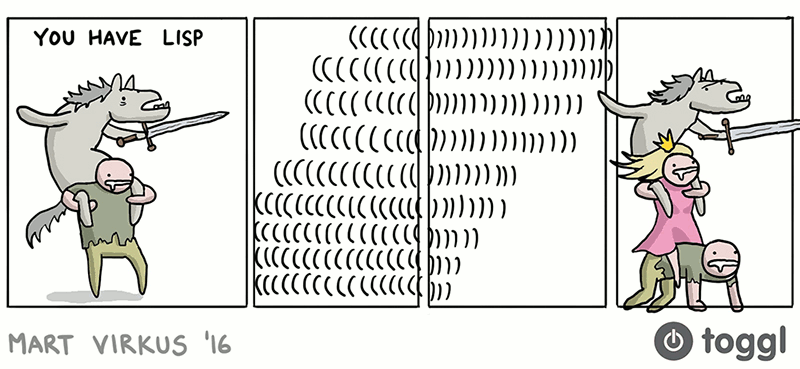
\includegraphics[width=\textwidth]{sulkeet.png}

\subsection{Funktionaalinen Clojure}
Clojure pyrkii olemaan funktionaalinen ohjelmointikieli, mutta epäpuhdas sellainen, sillä se ei pakota tekemään sovelluksista läpinäkyviä eikä todistettavissa olevia. Clojurella tehtyjä funktioita ei siis aina voida korvata arvoilla muuttamatta sovelluksen käyttäytymistä. Clojure sisältää myös laajan valikoiman mutatoitumattomia tietorakenteita (listoja, vektoreita, avain-arvo pareja).

\newpage
\section{Harjoitustyö}
Tehtävänannossa mainittiin, että ohjelmakoodin tulisi olla idiomaattista valitulle ohjelmointikielelle.
Emme ole täysin varmoja onko ohjelmakoodi täysin idiomaaattista mutta koska työn oli tarkoitus olla harjoitus funktionaaliseen paradigmaan,
toteutimme koodin niin, että siinä ei muuteta muuttujia ollenkaan.
Valitsimme Clojuren ohjelmointikieleksi koska ML:n kaltaisissa ohjelmointikielissä on liian vaikea syntaksi.

\subsection{Funktionaalisuuden hyödyt ja haitat}
Mielestämme ohjelmakoodin toteuttaminen funktionaalisesti oli vaikeampaa ja hitaampaa, kuin jos olisimme käyttäneet tavanomaisempaa
paradigmaa. Jo pelkästään silmukkarakenteiden tekeminen vaati paljon enemmän miettimistä. 


Pelitilaa ei ylläpidetä globaaleissa muuttujissa vaan se kulkee funktioiden parametreinä.
Tämän takia funktioiden rakentaminen oli hieman puhtaampaa koska mikään muu funktio ei voinut muuttaa tilaa joka oli saatu parametrinä.




\bibliographystyle{abbrv}
\bibliography{main}


\end{document}

